\section{QR-Codes}\label{chap:qrcodes}
Dieses Kapitel dreht sich um QR-Codes; allgemeine Informationen, wie werden eigentlich die Daten codiert beziehungsweise decodiert und wie läuft das überhaupt mit der Fehlerkorrektur?

\subsection{Allgemeines}
Wie bereits in Kapitel~\ref{chap:history} und \ref{chap:overview} erwähnt, wurde der QR-Code 1994 von der japanischen Firma \textit{DENSO Corporation} (gegründet 1949 als \textit{Nippondenso Co. Ltd.}) entwickelt. Wie der ausgeschriebene Name \textbf{Q}uick \textbf{R}esponse (schnelle Antwort) erwarten lässt, zeichnet sich der QR-Code vor allem durch die sehr schnelle Lesbarkeit aus. Diese ist in dem markanten Suchmuster des Codes begründet, welches gleichzeitig auch zur Lageerkennung verwendet wird.
Nachdem die Grundidee 1994 entwickelt worden war, wurde sie 1997 verbessert und im selben Jahr in der AIM\footnote{Automatic Identification and Mobility} Spezifikation ISS 97-001 beschrieben. Diese Spezifikation ist heute unter dem Namen QR-Code Model 1 bekannt. Ihr Hauptmerkmal ist eine immer schwarz gefärbte Zelle in der Ecke unten rechts, die von drei weißen Zellen umgeben ist (siehe Abbildung~\ref{fig:qrModel1}).\\
Im Jahr 2000 wurde dann eine überarbeitete Version des Codes in der ISO/IEC\footnote{International Organization for Standardization/International Electrotechnical Commission} Norm 18004:2000 beschrieben. Diese wurde umgangssprachlich als QR-Code Model 2 bezeichnet. Im Vergleich zu Model 1 besitzt das Model 2 die sechsfache Datenkapazität. Zudem wurden weitere Orientierungsmuster hinzugefügt, welche \zitext{wie kleine Suchmuster zur Ausrichtung des Referenzgitters im Code strukturiert verteilt sind.}{\cite{Lenk2012}}\\
\begin{figure}[htbp]
	\parbox{.47\textwidth}
	{
		\centering
		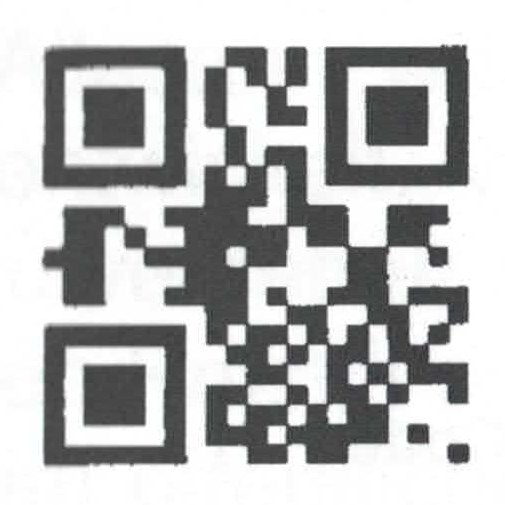
\includegraphics[height=2.5cm]{Bilder/QR_Code_Model_1.png}
		\caption[QR-Code Model 1]{QR-Code Model 1\footnotemark}
		\label{fig:qrModel1}
	}
	\hfill
	\parbox{.47\textwidth}
	{
		\centering
		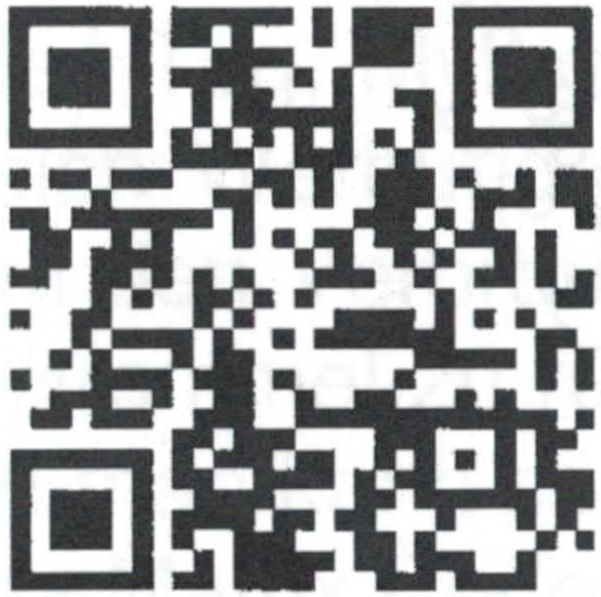
\includegraphics[height=2.5cm]{Bilder/QR_Code_Model_2.png}
		\caption[QR-Code Model 2]{QR-Code Model 2\textsuperscript{\ref{ftn:second}}}
		\label{fig:qrModel2}
	}
	\hfill
\end{figure}
\footnotetext{Quelle: \cite[3]{Lenk2012}\label{ftn:second}}~\\
Die heute verwendete Form des QR-Codes ist eine verbesserte Form des Model 2. 
Sie wurde 2006 in der Norm ISO/IEC 18004:2006 beschrieben und wird normalerweise als QR-Code 2005 (siehe Abbildung~\ref{fig:qr2005}) bezeichnet. 
2009 wurde sie um einige Detailverbesserungen ergänzt. 
In dieser Norm (18004:2006) wurde der normale QR-Code um den Micro QR-Code und den GS1 QR-Code erweitert. \pagebreak
Im weiteren Verlauf dieses Kapitels wird der QR-Code 2005 als Grundlage für alle weiteren Erläuterungen verwendet.

\begin{figure}[htbp]
	\centering
	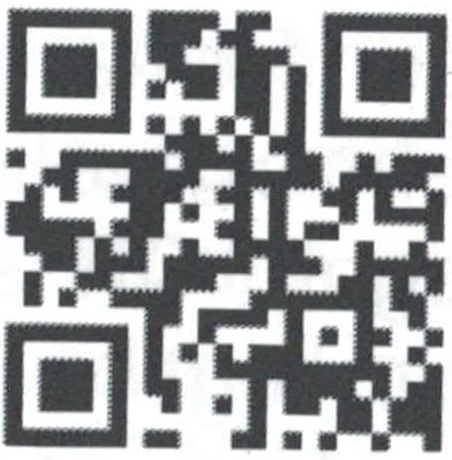
\includegraphics[width=2.5cm]{Bilder/QR_Code_2005.png}
	\caption[QR-Code 2005]{QR-Code 2005\footnotemark}
	\label{fig:qr2005}
	\hfill
\end{figure}
\footnotetext{Quelle: \cite[4]{Lenk2012}}

\subsection{Daten codieren}
Wie aber wird nun 

\pagebreak
